\documentclass[usepdftitle=false]{beamer}

\usepackage[T1]{fontenc}

\usepackage[utf8x]{inputenc}
\usepackage{default}
\usepackage{lmodern}
\usepackage{booktabs}

\usepackage{ragged2e} % Kommando\justifying ermöglicht  Blocksatz in Präsentationen

\mode<presentation>
 {\usecolortheme{seahorse,rose}
 \useinnertheme[shadow]{rounded}
%  \useoutertheme[hideothersubsections,right,width=4em,frame number]{sidebar}
%  \useoutertheme{infolines}
%\useoutertheme{split}
\useoutertheme[subsection=false,footline=authortitle]{miniframes}
\setbeamercovered{transparent}
}

%seitenzahl in linker ecke
\addtobeamertemplate{navigation symbols}{{\usebeamercolor{section
in toc}\footnotesize
\insertframenumber/\inserttotalframenumber}\hspace{48em}}{}
\usepackage{setspace} %mit spacing-Umgebung Zeilenabstand regeln



%%Sprachunterstuetzung
%Englische Silbentrennung, etc.
\usepackage[spanish]{babel}
%Mehrsprachige Literaturliste
\usepackage{babelbib}
%%Graphiken und Farbe
%Graphiken
\usepackage{graphicx} 
%von beamer.cls geladen
%Farbe
\usepackage{color,pgf}
%von beamer.cls geladen
%PDF-Seiten einbinden
\usepackage{pdfpages}
\usepackage{subscript}
\newcommand{\sub}[1]{\textsubscript{#1}}
\newcommand{\Sup}[1]{\textsuperscript{#1}}
\newcommand{\COO}{CO\textsubscript{2}}
\newcommand{\masl}{m~a.s.l.}
\newcommand{\gc}{$^{\circ}$C}
\newcommand{\tilt}{$\sim$}
\newcommand{\blue}[1]{{\color{blue!50!black}#1}}
\newcommand{\Blue}[1]{{\color{blue!50!black}\textbf{#1}}}
\newcommand{\eg}{e.\,g.}
\newcommand{\Eg}{E.\,g.}

% new environment for slides with changes margins
\newenvironment{changemargin}[2]{%
\begin{list}{}{%
\setlength{\topsep}{0pt}%
\setlength{\leftmargin}{#1}%
\setlength{\rightmargin}{#2}%
\setlength{\listparindent}{\parindent}%
\setlength{\itemindent}{\parindent}%
\setlength{\parsep}{\parskip}%
}%
\item[]}{\end{list}}





\hypersetup{
pdfauthor={Roman Link},
pdftitle={El sistema hidráulico de plantas},
}

%Titelseite
\title{El sistema hidráulico de plantas}
\subtitle{\normalfont Curso de laboratorio \textit{Mediciones de hidráulica de plantas con el XylEm Plus y la bomba de Scholander}}
\author[R. Link]{Roman Link}
\date{27 de noviembre de 2017}
\institute[University of Göttingen]{
Department of Plant Ecology and Ecosystem Research\\ Georg August University of Göttingen}
%\titlegraphic{ \vspace*{2em}
%
\includegraphics[width=0.7\textwidth]{logouni.png}}%oder was sch\"oneres

\logo{
\includegraphics[width=20em]{logounisolow.png}}

\usepackage{amsmath,amsfonts,amssymb,pgf}
 \usepackage { eulervm }

%\usepackage[round]{natbib}
%\def\newblock{} % hilft gegen absurde fehler mit natbib

\newcommand{\rar}{$\rightarrow$}
\newcommand{\lar}{$\leftarrow$}
\newcommand{\Rar}{$\Rightarrow$}
\newcommand{\Lar}{$\Leftarrow$}
\newcommand{\quelle}[1]{\baselineskip8pt{\tiny \color{gray} #1}}

\newcommand{\tw}{\textwidth}
\newcommand{\ddx}[2]{\frac{\mathrm{d}}{\mathrm{d}#2}#1 }
\newcommand{\ddxx}[2]{\frac{\mathrm{d^2}}{\mathrm{d}#2^2}#1}



\newcommand{\code}[1]{{\footnotesize \color{blue}
\texttt{#1}}\normalsize\color{black}}


% \input{cc_beamer}
\setbeamerfont{section in toc}{size=\normalsize,series=\bfseries}
\setbeamerfont{title}{series=\bfseries}
\setbeamerfont{frametitle}{size=\Large,series=\bfseries}

\begin{document}


%%%%%%%%%%%%%%%%%		Title Page			%%%%%%%%%%%%%%%%%%%%%%
\begin{frame}
\titlepage
\end{frame}

\begin{frame}
 \frametitle{Estructura de la presentación}
\tableofcontents
%\begin{itemize}
% \item \Blue{8:00} 
%\end{itemize}
\end{frame}


%%%%%%%%%%%%%%%%%%%%%%%%%%%%%%%%%%%%%%%%%%%%%%%%%%%%%%%%%%%%%%%%%%%%%%%%%%%%%%%%%%%%%%
\section[Transporte de agua]{Transporte de agua en plantas} 
%%%%%%%%%%%%%%%%%%%%%%%%%%%%%%%%%%%%%%%%%%%%%%%%%%%%%%%%%%%%%%%%%%%%%%%%%%%%%%%%%%%%%%

\begin{frame}
	\frametitle{Funciones de agua en plantas}
		\begin{itemize}[<+->]
		\item Medio fluido del citoplasma: entorno para reacciones bioquímicas
		\item Transporte de nutrientes disueltos de las raíces hasta las hojas
		\item Fotosíntesis (6 CO$_2$ + \Blue{6 H$_2$O} → C$_6$H$_{12}$O$_6$ + 6O$_2$)
	\end{itemize}
	
	\vspace{0.5em}
	\visible<4>{
    \centering{
    \begin{minipage}{0.7 \tw}    	
    	\begin{block}{\textbf{Área de investigación:\\ relaciones de agua de plantas}}
    		Estudios de las estrategias de plantas para estabilizar su balance de agua	
    	\end{block}
    \end{minipage}}}
\end{frame}

\begin{frame}
	\frametitle{¿Son plantas ineficientes en su uso de agua?}
	\begin{itemize}
		\item<1- |alert@1> Alrededor de 90\% de la agua usada por una planta están perdidos por transpiración para poder absorber CO$_2$ (Kramer \& Boyer, 1995)
		\item<2- |alert@2> 1 g de material orgánico \lar\ ca. 500 g de agua
		\item<visible@3 |alert@3>[\Rar] Productividad de plantas depende de la disponibilidad de agua
	\end{itemize}
\end{frame}

\begin{frame}
	\frametitle{Transporte de agua en el xilema}
	\begin{changemargin}{-2em}{-2em}
		\begin{minipage}{0.52 \paperwidth}
			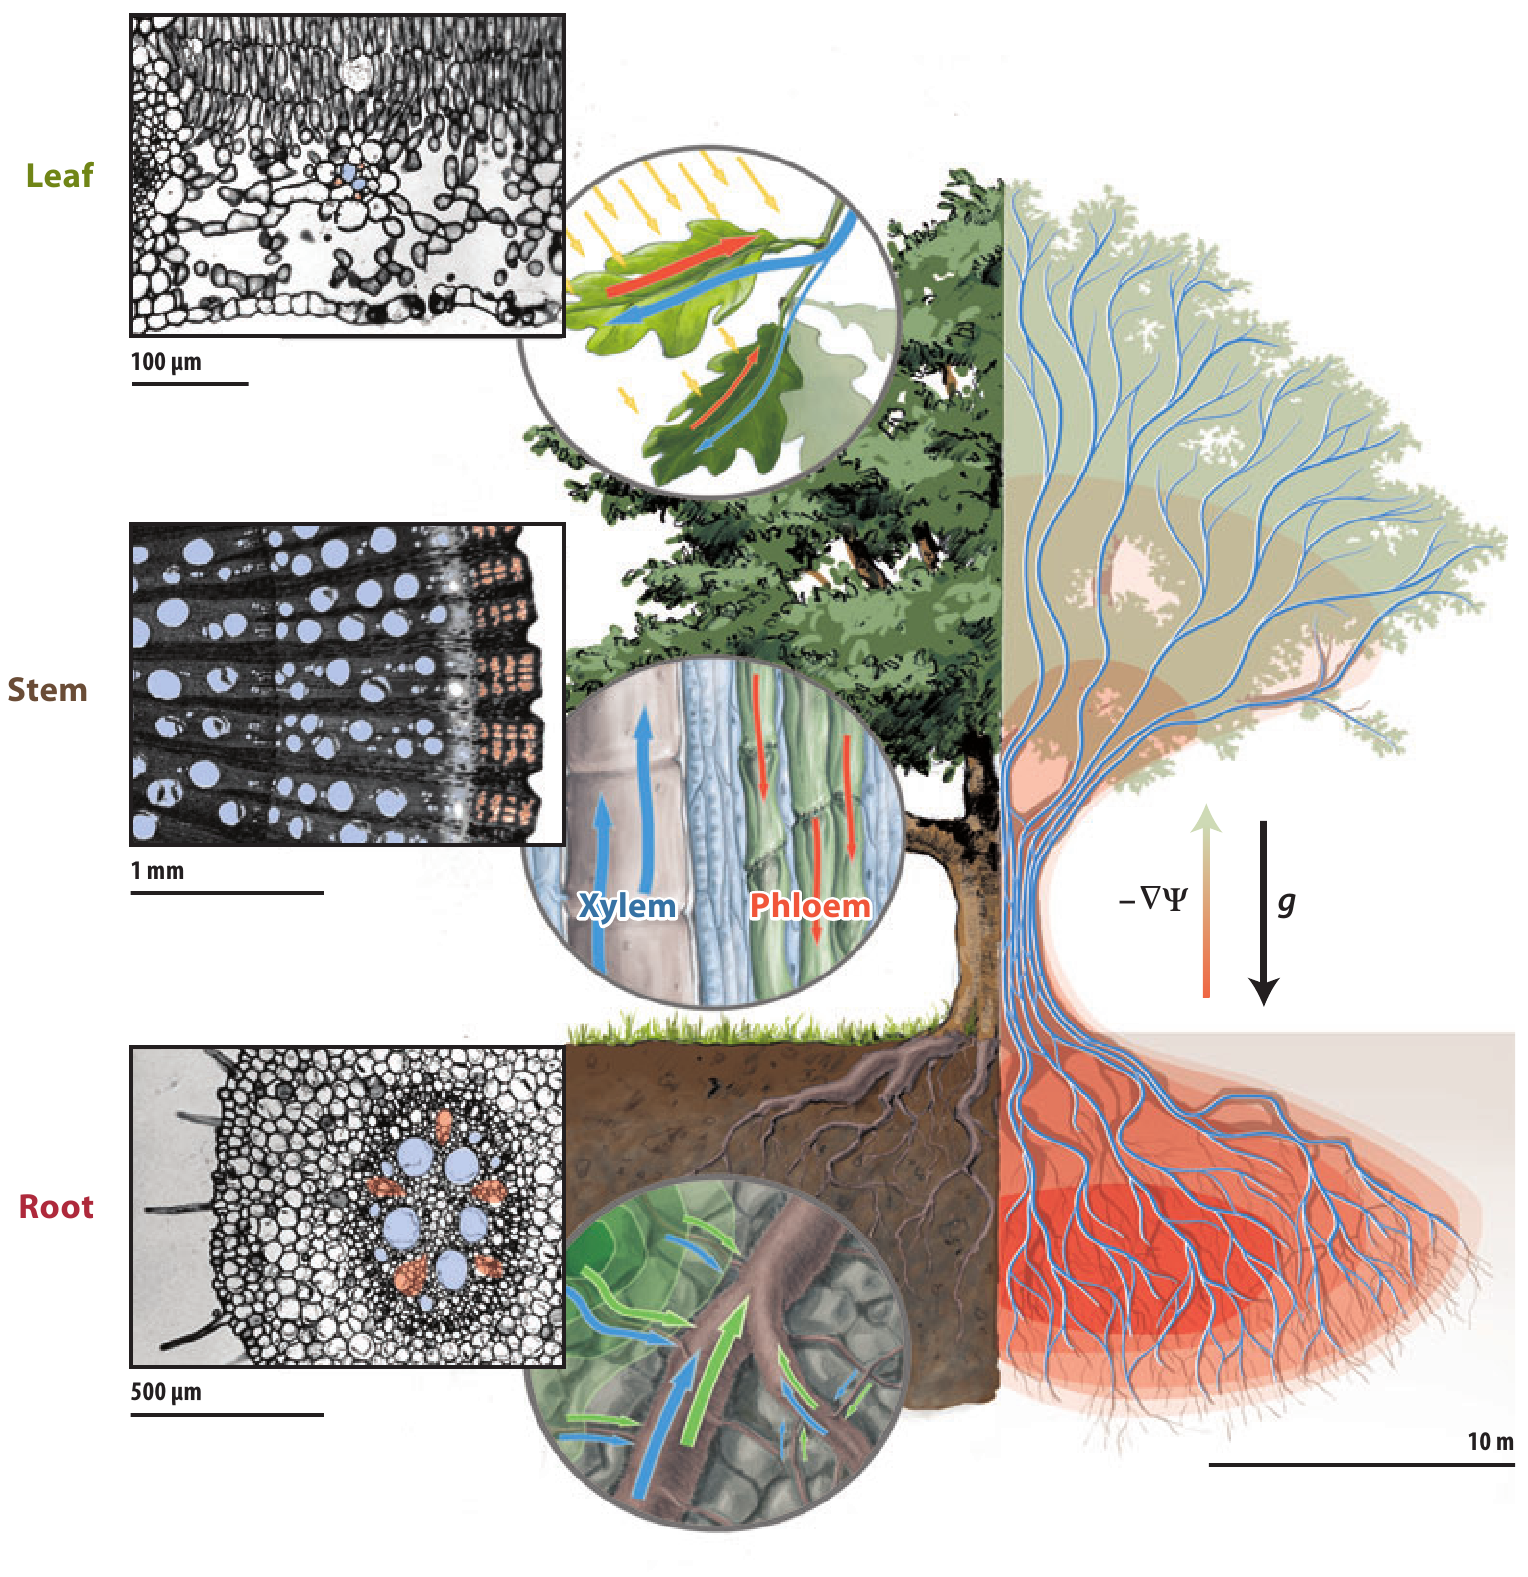
\includegraphics[width = \tw]{pictures/stroock_watertrans.png}\\
			\centering{\quelle{\textbf{Ilustración:} Stroock et al., 2014}}
		\end{minipage}
		\begin{minipage}{0.4 \paperwidth}
			\small
			\begin{itemize}
				\item<1-> Fuerza impulsora del transporte de agua en plantas:\alert<1>{\textbf{VPD} (déficit de presión de vapor)} 
				\item<2-> \alert<2>{Mecanismo de cohesión y tensión}: columnas continuas de agua desde las raíces hasta las hoja
				\item<visible@3-| alert@3> [\rar]Líquido bajo presión negativa: \textbf{estado meta-estable}
				\item<visible@4| alert@4> [\rar]Si la presión se vuelve demasiado negativa:\\ \textbf{riesgo de embolias \&\\ perdida de conductividad}
			\end{itemize}
		\end{minipage}
	\end{changemargin}
\end{frame}

\begin{frame}
\begin{block}{\textbf{El déficit de presión de vapor (VPD)}}
	\begin{itemize}
	 \item<1-> Diferencia entre la presión de vapor saturado ($VP_{sat}$) y la presión de vapor actual ($VP_{air}$)
	 \end{itemize}
	 
	 	\vspace{-1em}
	 	\begin{equation*}
	 	VPD = VP_{sat} - VP_{air}
	 	\end{equation*}
	 	
		\vspace{-1em}
   	\begin{itemize}
	 \item $VP_{air}$ se puede calcular a base de la humedad relativa ($rh$)
	 \end{itemize}
	 
	\vspace{-2em}	
	\begin{align*}
		VPD &= VP_{sat}  - VP_{sat} \cdot rh/100 \\
		    &= VP_{sat} \cdot (1 - rh/100) 
	\end{align*}
	
	\vspace{-1em}
	\begin{itemize}
		\item<2-> $VP_{sat}$ depende directamente de la temperatura
		\item<visible@3>[\Rar] \alert{La temperatura determina la demanda transpirativa de plantas}
	\end{itemize}
\end{block}
\end{frame}


%%%%%%%%%%%%%%%%%%%%%%%%%%%%%%%%%%%%%%%%%%%%%%%%%%%%%%%%%%%
\section{El potencial hídrico}
%%%%%%%%%%%%%%%%%%%%%%%%%%%%%%%%%%%%%%%%%%%%%%%%%%%%%%%%%%%
\begin{frame}
	\frametitle{El potencial hídrico}
	\begin{changemargin}{-2em}{-2em}
		\begin{minipage}{0.5 \paperwidth}
				\begin{block}{\textbf{Potencial hídrico}}
				La energía potencial de agua por unidad de volumen en relación a agua pura en condiciones de referencia
			\end{block}
			\begin{itemize}
				\item<2- |alert@2> Concepto muy útil para analizar el flujo de agua en el \textbf{continuo de suelo, planta y atmósfera}
				\item<3- |alert@3> Flujo siempre dirigido hacia potenciales más negativos
				\item<4- |alert@4> Transporte completamente pasivo, basado en principio de equilibrio
			\end{itemize}
			\centering{\quelle{\textbf{Ilustración:} Campbell \& Reece, 2006}}
		\end{minipage}		
		\begin{minipage}{0.42 \paperwidth}
			\vspace{-3em}
			\hspace{1.6em}
			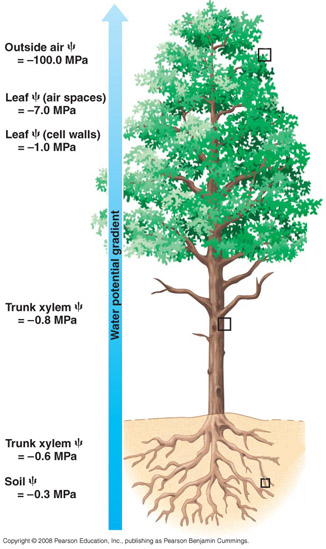
\includegraphics[width = \tw]{pictures/campbell_reese_2006.jpg}\\
		\end{minipage}
	\end{changemargin}    
\end{frame}

\begin{frame}
	\frametitle{Componentes del potencial hídrico}
	{\huge
	\begin{equation*}
	\Psi = \Psi_0 + \Psi_\pi + \Psi_p + \Psi_s + \Psi_v + \Psi_m
	\end{equation*}}
	\begin{description}
		\item[$\Psi_0$] Potencial de referencia
		\item[$\Psi_\pi$] Componente osmótico
		\item[$\Psi_p$]   Componente presión
		\item[$\Psi_s$]   Componente gravitacional
		\item[$\Psi_v$]   Potenciál en relación a la humedad
		\item[$\Psi_m$]   Potencial según fuerzas mátricas (cohesión, capilaridad \& tensión superficial)
	\end{description}
	\visible<2>{\textbf{\alert{El potencial hídrico se expresa en unidades de presión (MPa)}}}
\end{frame}


\begin{frame}
	\frametitle{Componentes del potencial hídrico}
	\textbf{\Large Ejemplos}
	\begin{itemize}
		\item \Blue{Potencial osmótico $\Psi_\pi$:} Potenciales en dependencia de la concentración $c$ de una sustancia en solución
		\begin{itemize}
		    \item $c = 0.01~mol~L^{-1}$ \rar\ $\Psi_\pi = -0.027~MPa$
			\item $c = 1.00~mol~L^{-1}$  \rar\ $\Psi_\pi = -2.270~MPa$			 
		\end{itemize} 
	    \item \Blue{Potencial de presión $\Psi_p$:}
	    \begin{itemize}
	    	\item Turgencia: positivo
	    	\item Tensión: negativo	 
	    	\item[\Rar] Presión hidrostática
	    \end{itemize} 
	    \item \Blue{Potencial gravitacional $\Psi_s$:} \begin{itemize}
	    	\item[] $\Psi_g = \rho \cdot g \cdot h \approx\ 0.01~MPa\,m^{-1}$ 
	    \end{itemize} 
	\end{itemize}
\end{frame}


\begin{frame}
	\frametitle{Componentes del potencial hídrico}
\textbf{Las tres componentes más importantes para el movimiento de agua en plantas a largas distancias:}
		\begin{itemize}
			\item Presión de raíces (potencial osmótico)
			\item Capilaridad (potencial mátrico)
			\item Transpiración	 (potencial de presión)		
		\end{itemize}

\end{frame}

\begin{frame}
	\frametitle{Mediciones de potenciales hídricos}
		\begin{block}{\textbf{Bomba de Scholander}}
		\centering{
			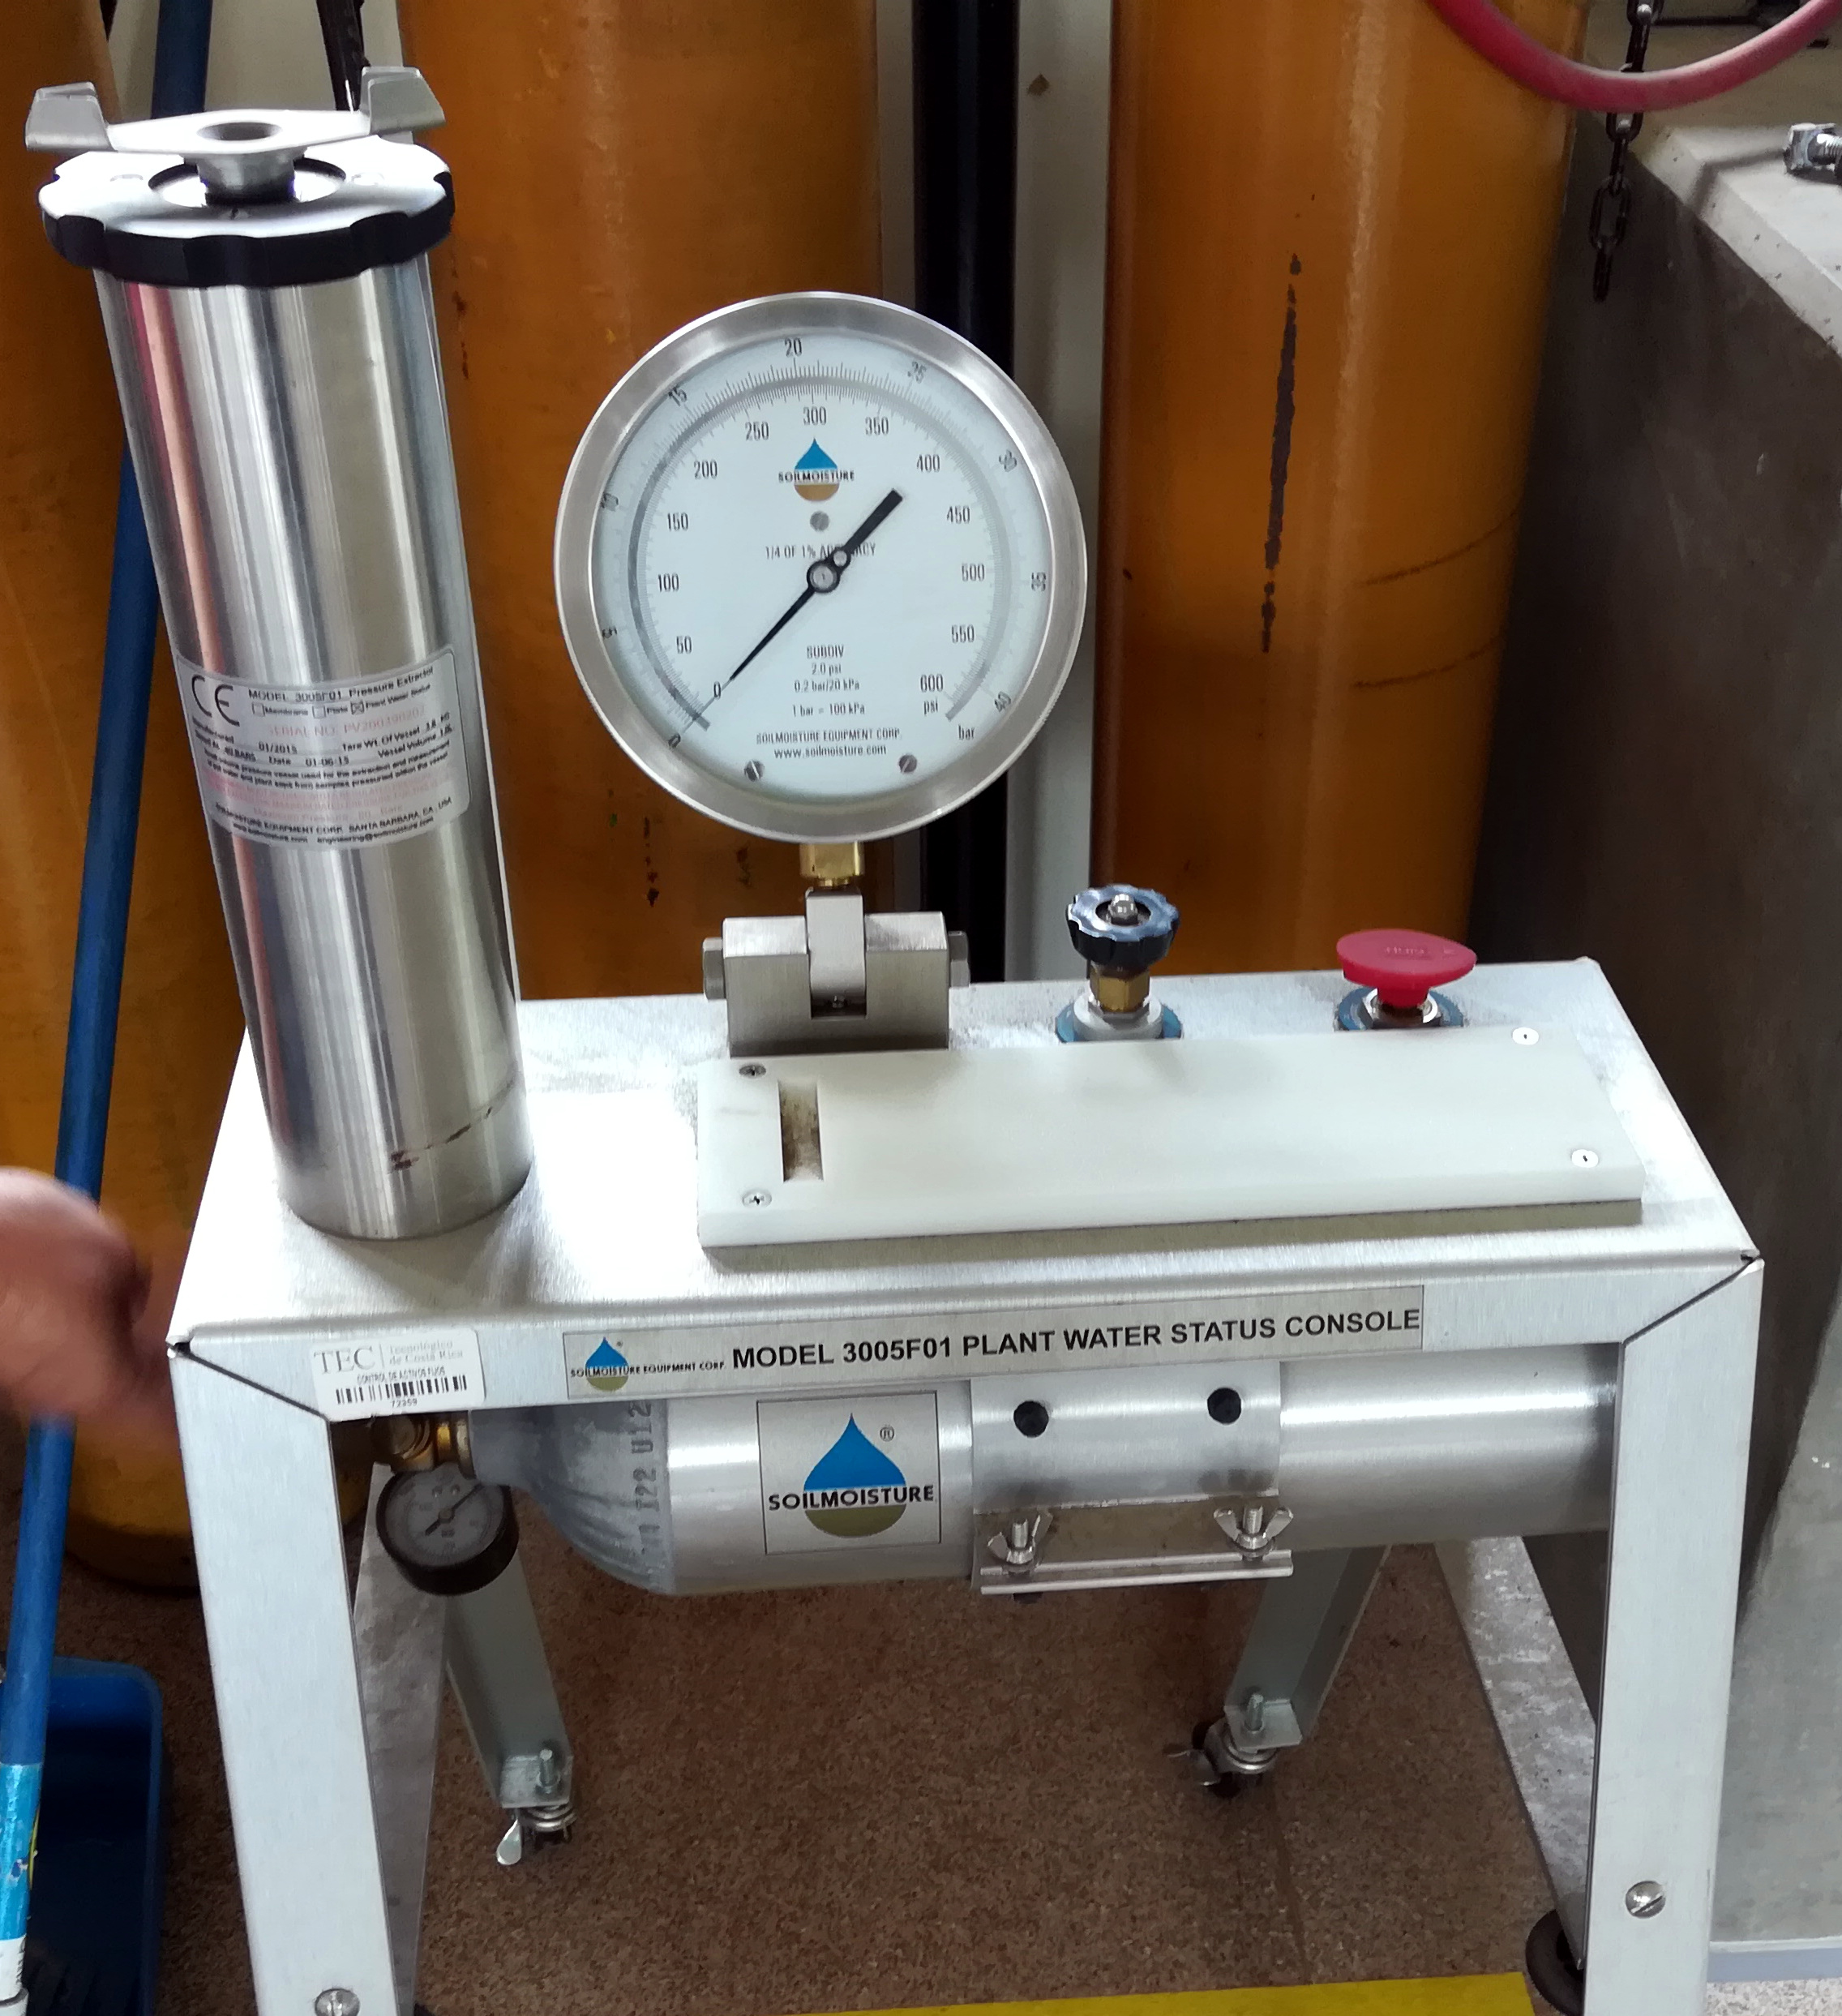
\includegraphics[height =0.5\tw]{pictures/bomba1.jpg}
			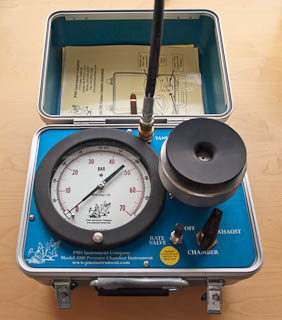
\includegraphics[height =0.5\tw]{pictures/bomba2.jpg}
	     	}
		\end{block}
\end{frame}


%%%%%%%%%%%%%%%%%%%%%%%%%%%%%%%%%%%%%%%%%%%%%%%%%%%%%%%%%%%%%%%%%%%
\section{Conductividad hidráulica}
%%%%%%%%%%%%%%%%%%%%%%%%%%%%%%%%%%%%%%%%%%%%%%%%%%%%%%%%%%%%%%%%%%%

\begin{frame}
	\frametitle{Conductividad hidráulica}
	\begin{block}{\textbf{Pregunta de motivación:}}
      	\begin{itemize}
			\item<+-| alert@+> ¿Si la productividad depende de la disponibilidad de agua, porque las plantas no simplemente maximizan la cantidad de agua que llega a las hojas?
			\item<+-| alert@+>  ¿\textbf{Conductividad} más alta \rar\ más crecimiento?
		\end{itemize}
    \end{block}
\end{frame}



\begin{frame}
	\frametitle{Conductancia y conductividad}
\textbf{\Large Tres definiciones importantes:}
		\begin{itemize}
			\item \Blue{Conductancia} \\
			
		    \vspace{0.3em}			
			{\Large $\frac{\mathrm{Tasa\ de\ flujo}}{\mathrm{Gradiente\ de\ presión}} \Big[\frac{kg/s}{MPa}\Big]$}
			
		    \vspace{0.5em}
			\item \Blue{Conductividad hidráulica} 			
			
			\vspace{0.3em}	
			{\Large$\frac{\mathrm{Tasa\ de\ flujo\ \cdot\ Longitud\ de\ muestra}}{\mathrm{Gradiente\ de\ presión}} 			\Big[\frac{kg/s}{MPa} \cdot m\Big]$}
			
					    \vspace{0.5em}
			\item \Blue{Conductividad específica}			
			
			\vspace{0.3em}	
			{\Large $\frac{\mathrm{Tasa\ de\ flujo}}{\mathrm{Gradiente\ de\ presión}} \cdot \frac{\mathrm{Longitud\ de\ muestra}}{\mathrm{Área\ conductiva}}\Big[\frac{kg/s}{MPa} \cdot \frac{m}{m^2}\Big]$}
		\end{itemize}

\end{frame}

\begin{frame}
	\frametitle{¿De qué depende la conductividad del xylem?}
	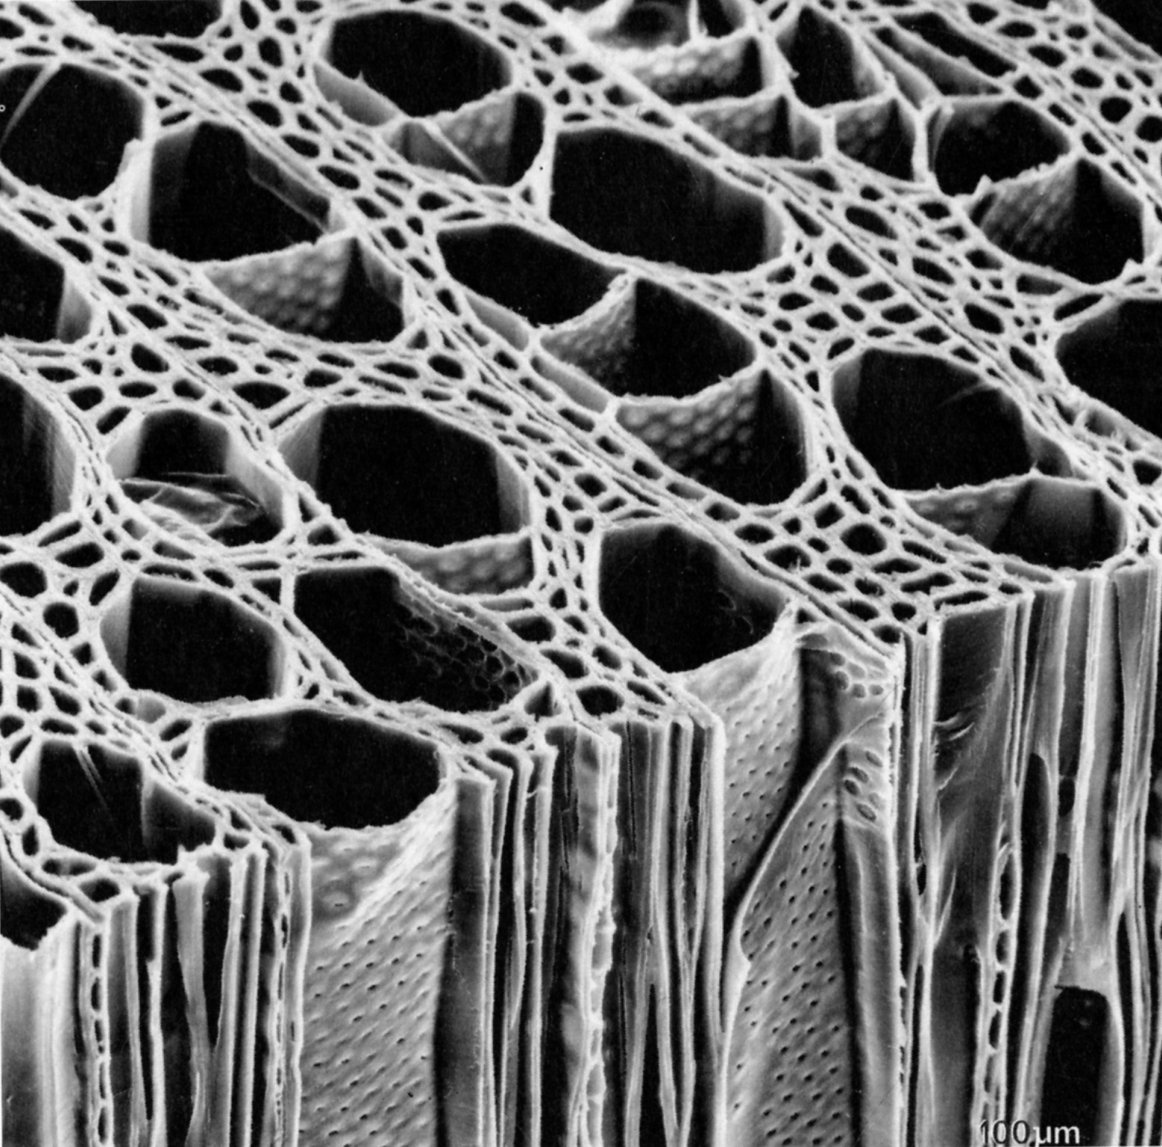
\includegraphics[height = 0.5 \textheight]{pictures/tyree_zimmermann_2003_2.jpg}
	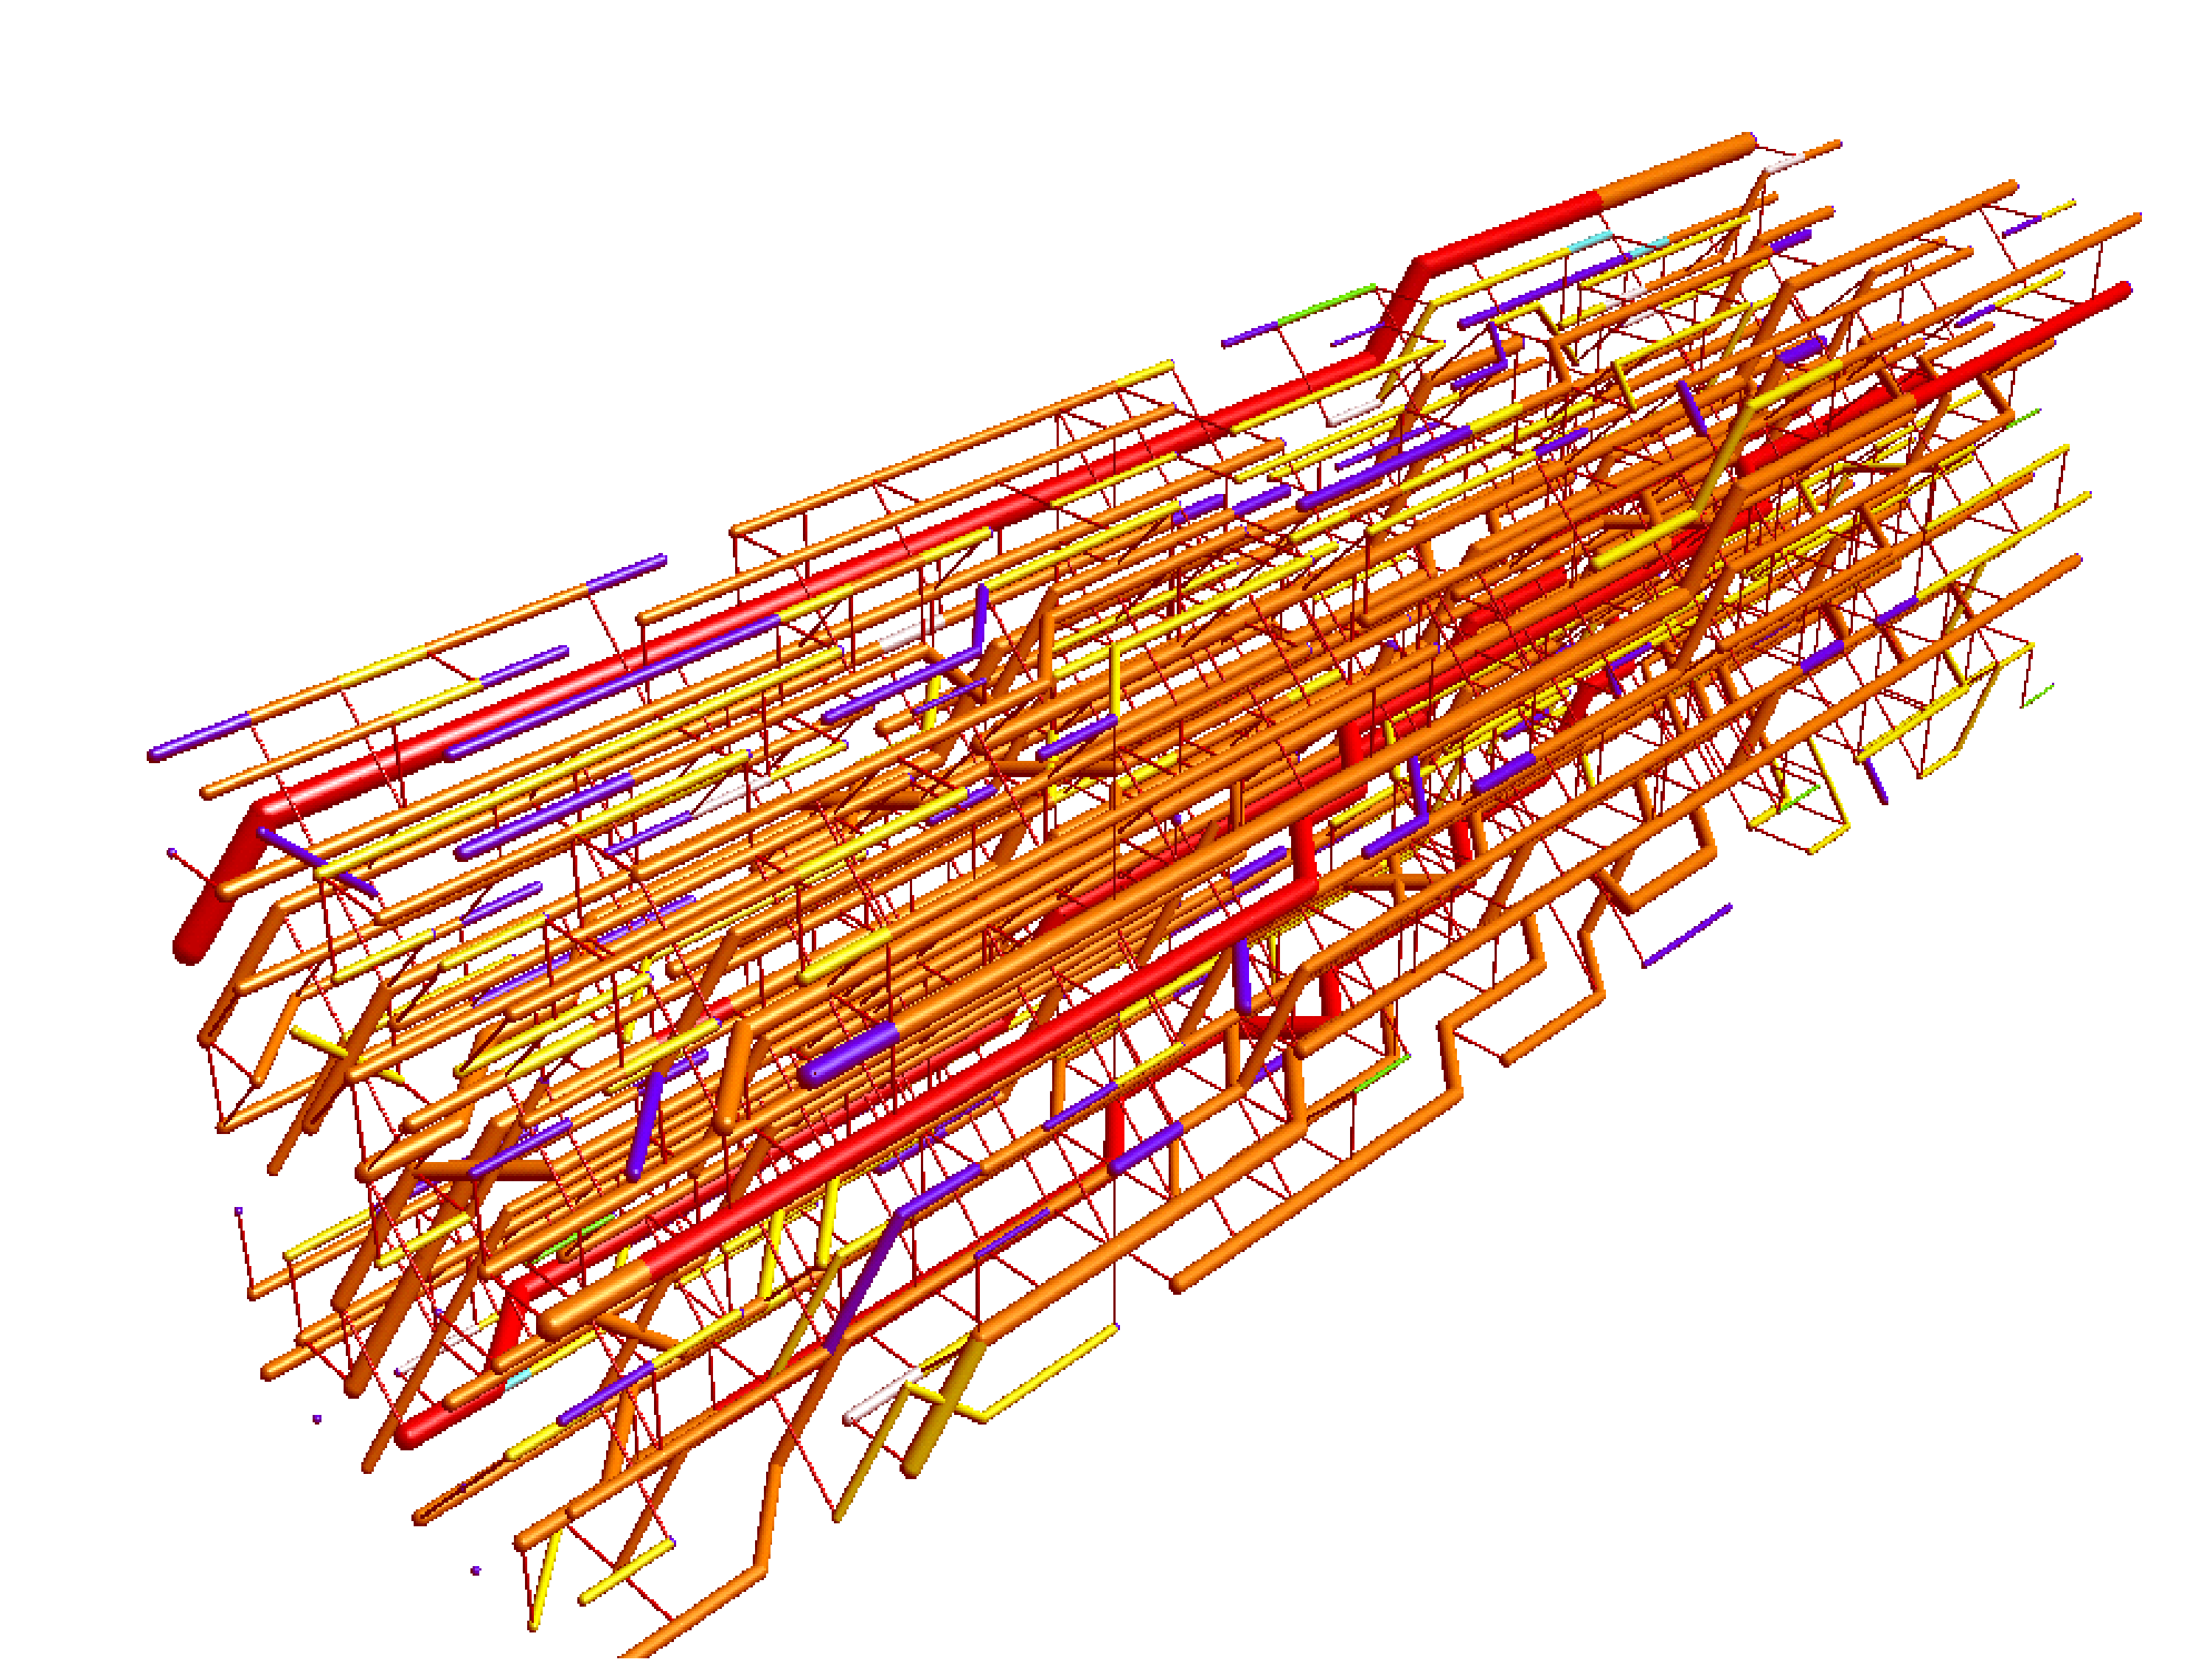
\includegraphics[height = 0.6 \textheight]{pictures/tyree_zimmermann_2003_1.png}\\

	\begin{itemize}
		\item Estructura del xylem: red compleja de traqueidas (y vasos en caso de angiospermos) interconectad@s					
	\end{itemize}
	\centering{\quelle{\textbf{Ilustración: Tyree \& Zimmermann, 2003}}}
\end{frame}
		
\begin{frame}
	\frametitle{¿De qué depende la conductividad del xylem?}
	\begin{minipage}{0.3 \tw}
        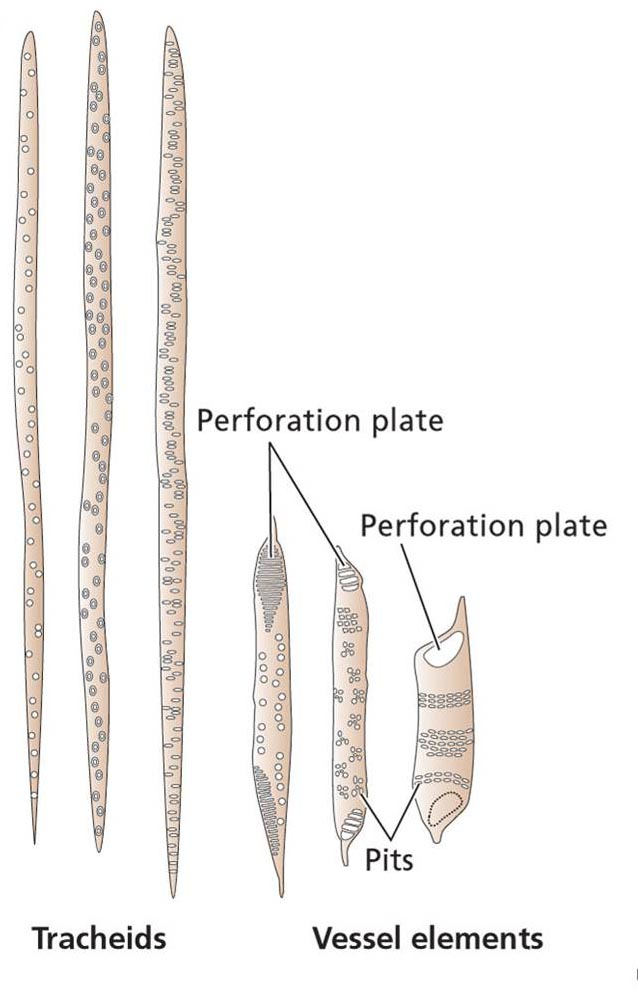
\includegraphics[width = \tw]{pictures/taiz_zeiger_2000.jpg}
	\end{minipage}
		\begin{minipage}{0.68 \tw}
			\begin{itemize}	
				\item Flujo en el lumen de vasos/traqueidas - \alert{Ecuación de Hagen-Poiseuille} (flujo en capilares ideales):
				\item[] {\huge $F = \frac{\pi \cdot \alert<2>{r^4}}{8\eta} \cdot \frac{\Delta \Psi_p}{l} $}
				\begin{description}
					\item[\Blue{$\eta$}] Viscosidad dinámica
					\item[\Blue{$l$}] Longitud del capilar
				\end{description}
				\item<visible@2> \alert{Conductividad aumenta con $r^4$}
			\end{itemize}			
		\end{minipage}	
				\centering{\quelle{\textbf{Ilustración: Taiz \& Zeiger, 2002}}}
\end{frame}


\begin{frame}
\frametitle{¿De qué depende la conductividad del xylem?}
\begin{minipage}{0.2 \tw}
	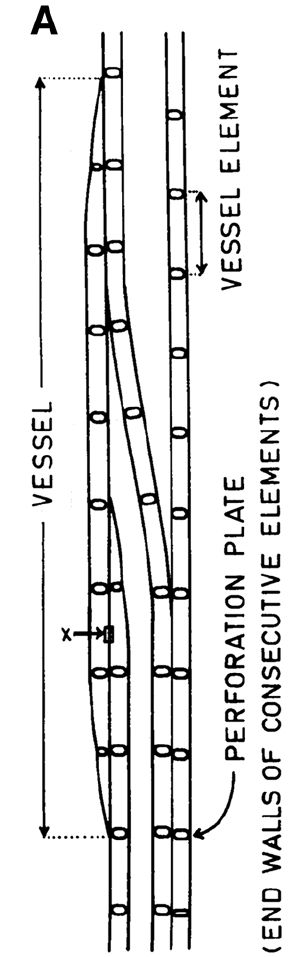
\includegraphics[width = \tw]{pictures/zimmermann_in_cai_vesselconcept.png}
\end{minipage}
\begin{minipage}{0.78 \tw}
	\centering{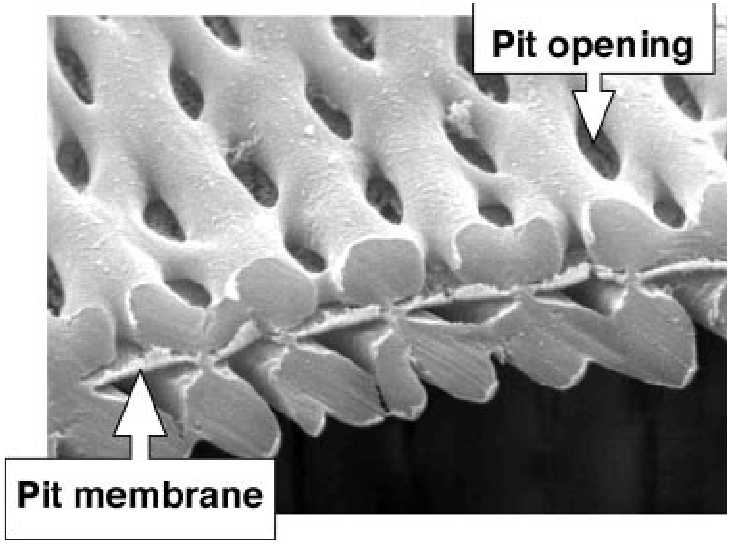
\includegraphics[width = 0.6\tw]{pictures/hacke01_pit_membranes.png}}	
	\begin{itemize}	
		\item Transición de un(a) vaso/traqueída a otr@:\\
		\begin{itemize}
			\item<1-> \alert<1>{Resistencia de flujo} de punteaduras 
			\item<2-> \alert<2>{Densidad de punteaduras}
			\item<3-> Además importante: \alert<3>{Longitud de vasos} (vasos cortos: más punteaduras en el camino del agua)
		\end{itemize}		
	\end{itemize}			
\end{minipage}	
\centering{\quelle{\textbf{Ilustración: izquierda - Zimmermann \& McDonough, 1978; derecha - Hacke \& Sperry, 2001}}}
\end{frame}	

\begin{frame}
	\frametitle{La formación de embolias}
    \centering{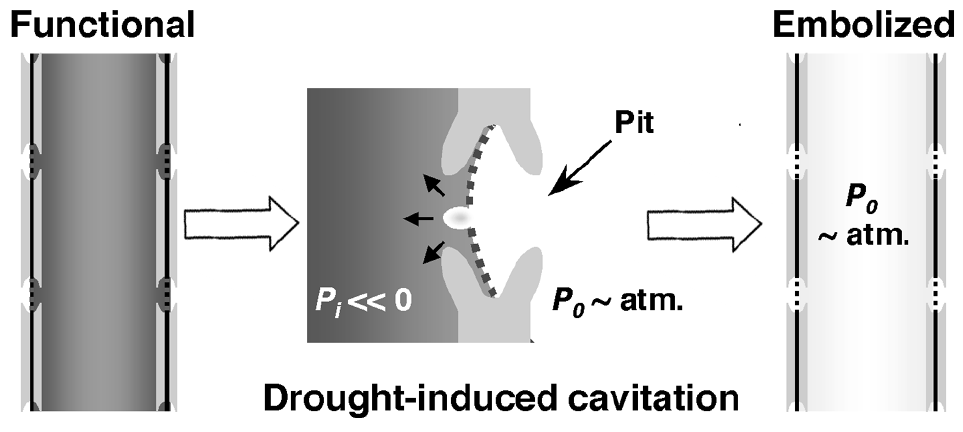
\includegraphics[width =0.7\tw]{pictures/hacke01_air_seeding1.png}}
  \begin{itemize}
  \item Embolias están causadas por aire entrando por poros inusualmente grandes en las membranas de las punteaduras
  \item El riesgo de embolias está relacionado a la densidad, el grosor y el área total de punteaduras
  \end{itemize}
{\raggedright \quelle{\textbf{Ilustración:}  Hacke \& Sperry, 2001 (modificado)}}
\end{frame}

\begin{frame}
	\frametitle{Stability-efficiency-tradeoff}
	\begin{itemize}
			\item \textbf{Para optimizar eficiencia conductiva, una planta tiene que\dots}
			\begin{itemize}
				\item<1-| alert@1> \dots aumentar diámetro y longitud de vasos
				\item<2-| alert@2> \dots aumentar densidad de punteaduras
				\item<3-| alert@3> \dots bajar resistencia de flujo de las punteaduras (aumentar diámetro)
			\end{itemize}
			
			\item<visible@4-> \textbf{PERO: Para optimizar seguridad contra embolías, una planta tiene que\dots}
			\begin{itemize}
				\item<4-| alert@4> \dots bajar diámetro y longitud de vasos
				\item<5-| alert@5> \dots bajar densidad de punteaduras
				\item<6-| alert@6> \dots aumentar resistencia de flujo de las punteaduras (bajar diámetro)
			\end{itemize}			
			\item<visible@7-| alert@7>[\Rar] \textbf{Plantas no pueden maximizar conductividad hidráulica y resistencia contra sequía al mismo tiempo}					
	\end{itemize}
\end{frame}

\begin{frame}
	\frametitle{Mediciones de conductividad}
	\centering{
		\begin{minipage}{0.6\tw}
			\begin{block}{\textbf{XylEm Plus}}
				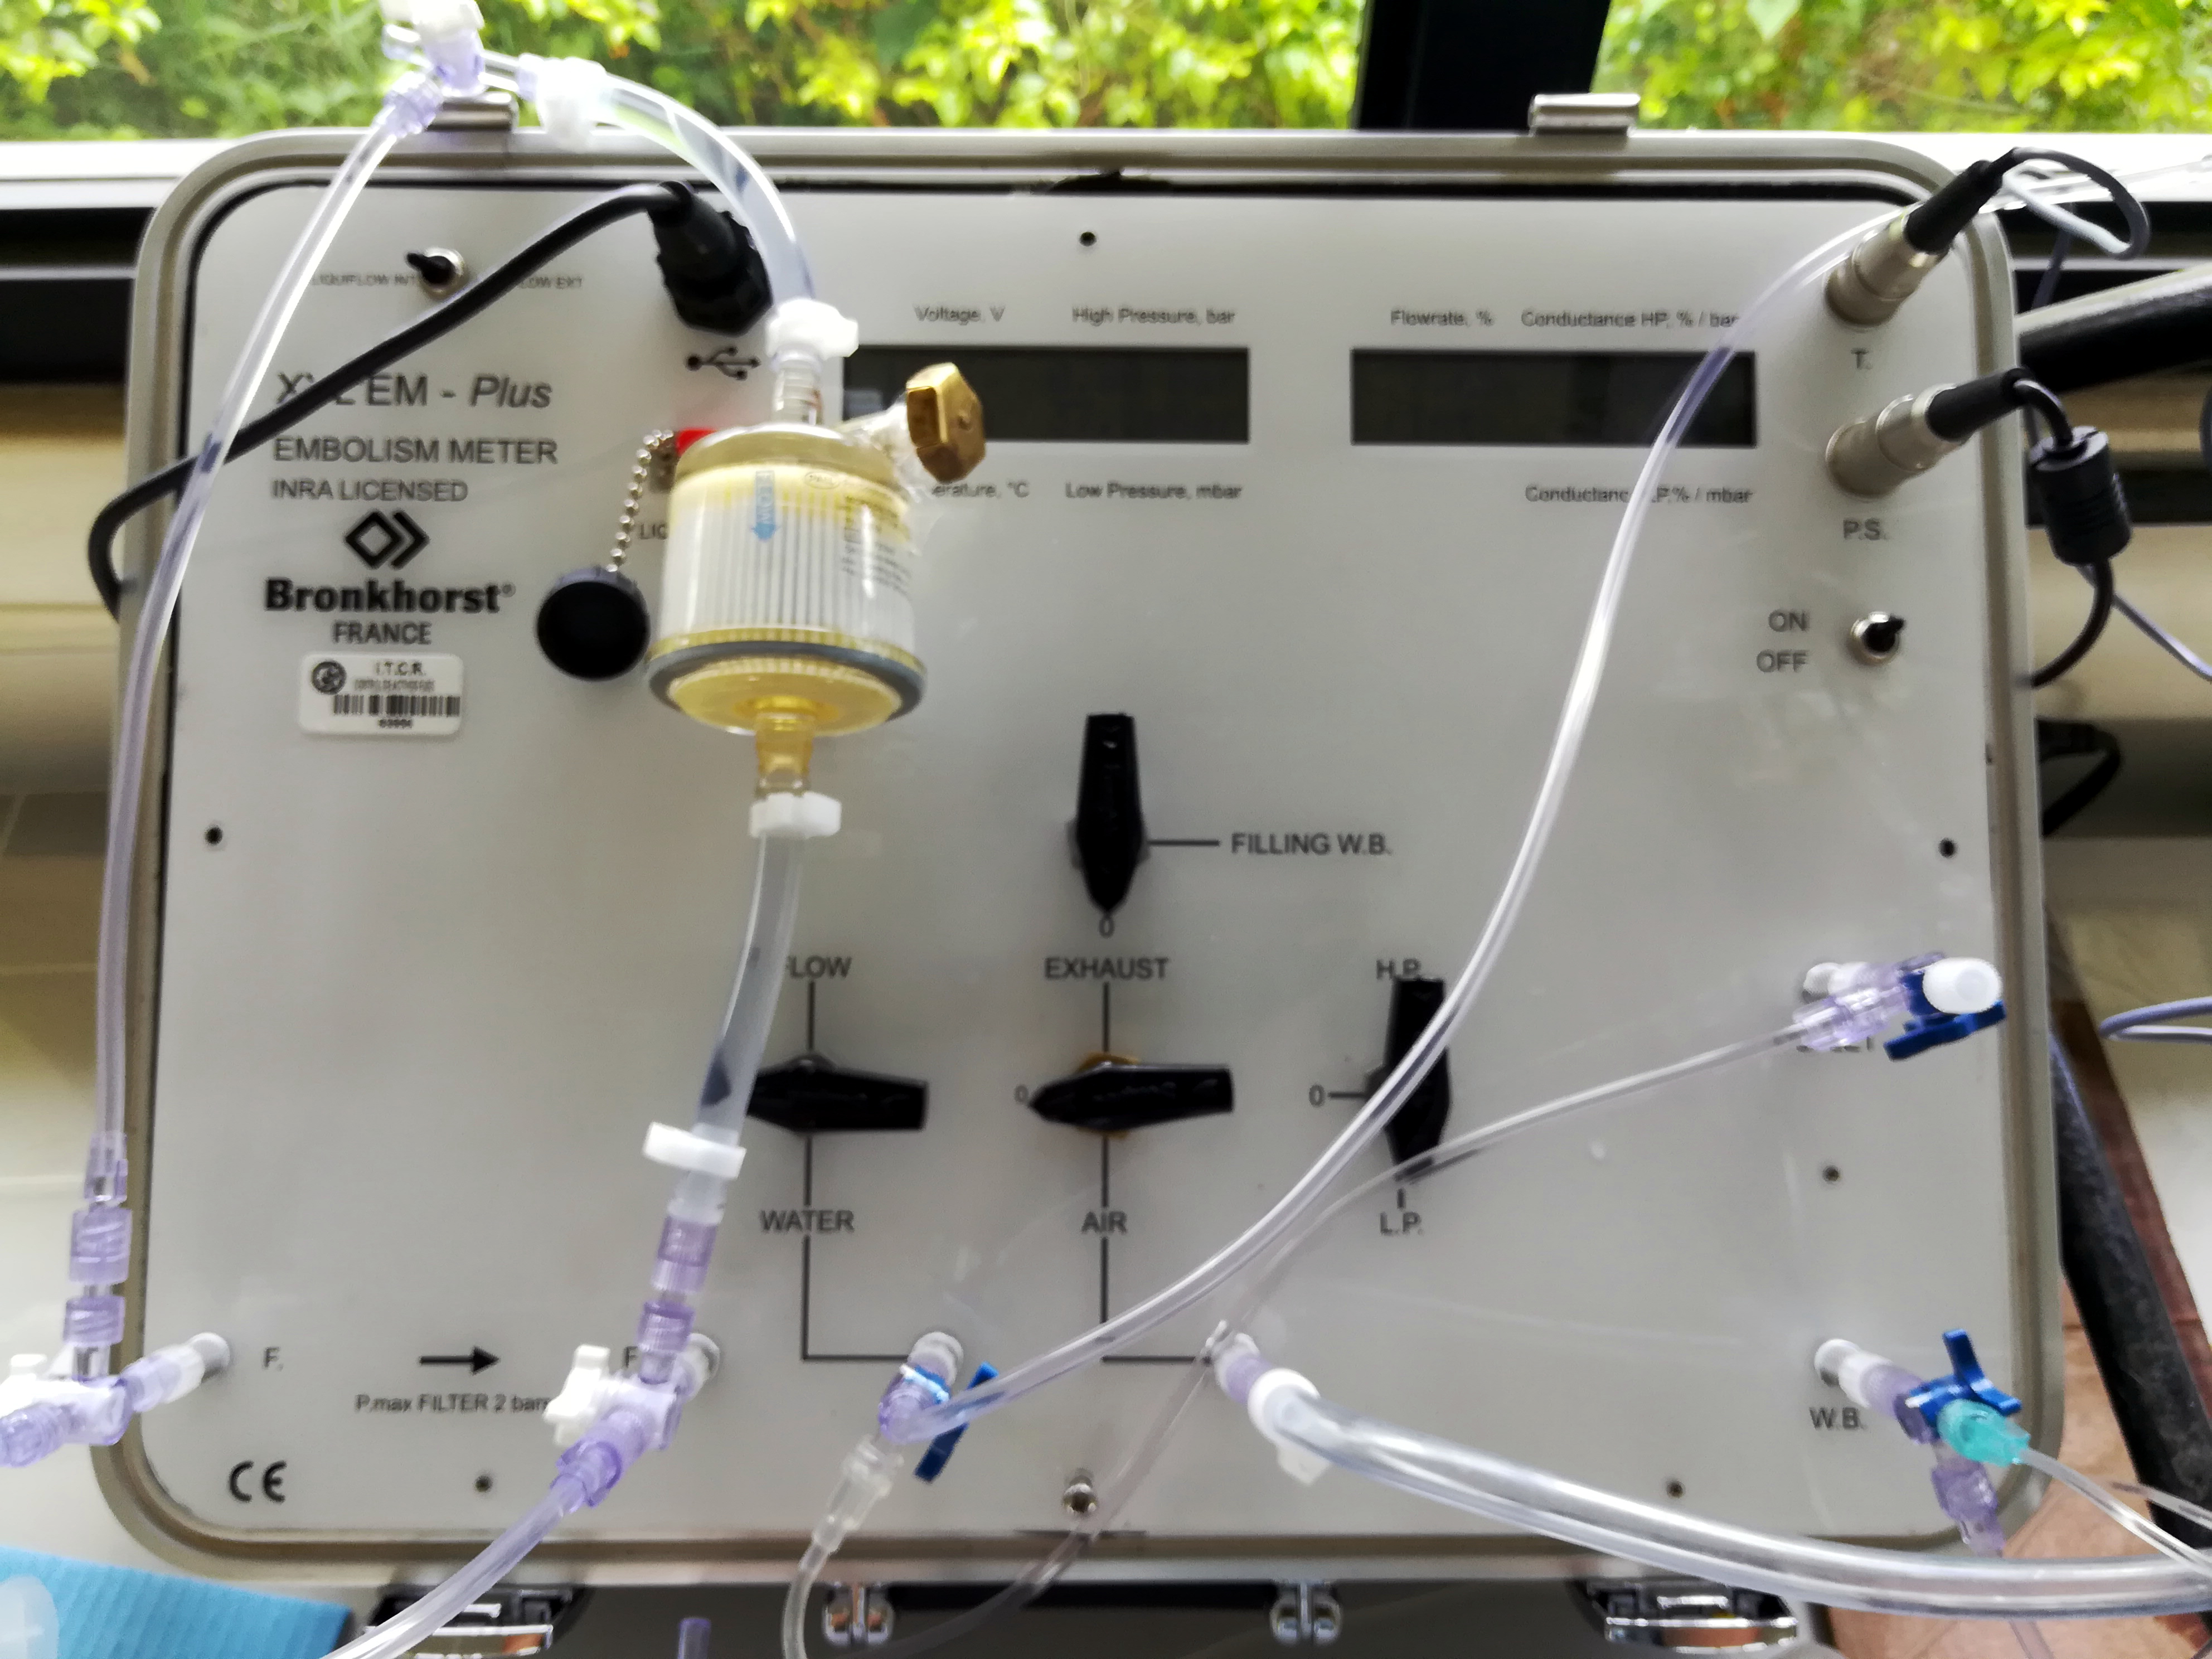
\includegraphics[width =\tw]{pictures/xylem.jpg}			
			\end{block}
		\end{minipage}}
	\end{frame}


%%%%%%%%%%%%%%%%%%%%%%%%%%%%%%%%%%%%%%%%%%%%%%%%%%%%%%%%%%%%%%%%%%%%
\section{Curvas de vulnerabilidad}
%%%%%%%%%%%%%%%%%%%%%%%%%%%%%%%%%%%%%%%%%%%%%%%%%%%%%%%%%%%%%%%%%%%%
\begin{frame}
	\begin{block}{\textbf{Estrategias hidráulicas}}
	\begin{itemize}
		\item Cada especie de planta posee una\textbf{ estrategía hidráulica} propia que está definiendo su posición entre el espacio definido por seguridad y eficiencia
		\item \textbf{Hidráulica de plantas} es la ciencia que está analizando estas estrategías para entender  cuales son los beneficios de estrategías diferentes para una especie bajo diferentes condiciones ambientales, y como afectan su mortalidad en un clima cambiando		
	\end{itemize}
	\end{block}
\end{frame}



\begin{frame}
	\frametitle{Variables medidos en este curso}

	   \begin{minipage}{0.68 \tw}
         	\begin{itemize} 
         		\item \Blue{Potencial hídrico:} Estado de agua actual de las hojas 
         		\item[\rar]medido con bomba de Scholander 
         		\item \Blue{Conductividad:} Capacidad de transportar  agua hacia las hojas
         		\item[\rar] medido con XylEm Plus o aparato de Sperry		
         		\item<visible@2| alert@2> Relación entre conductividad y potencial hídrico: \textbf{Curva de vulnerabilidad}
         	\end{itemize}	 
	   \end{minipage}
		\begin{minipage}{0.3\tw}
          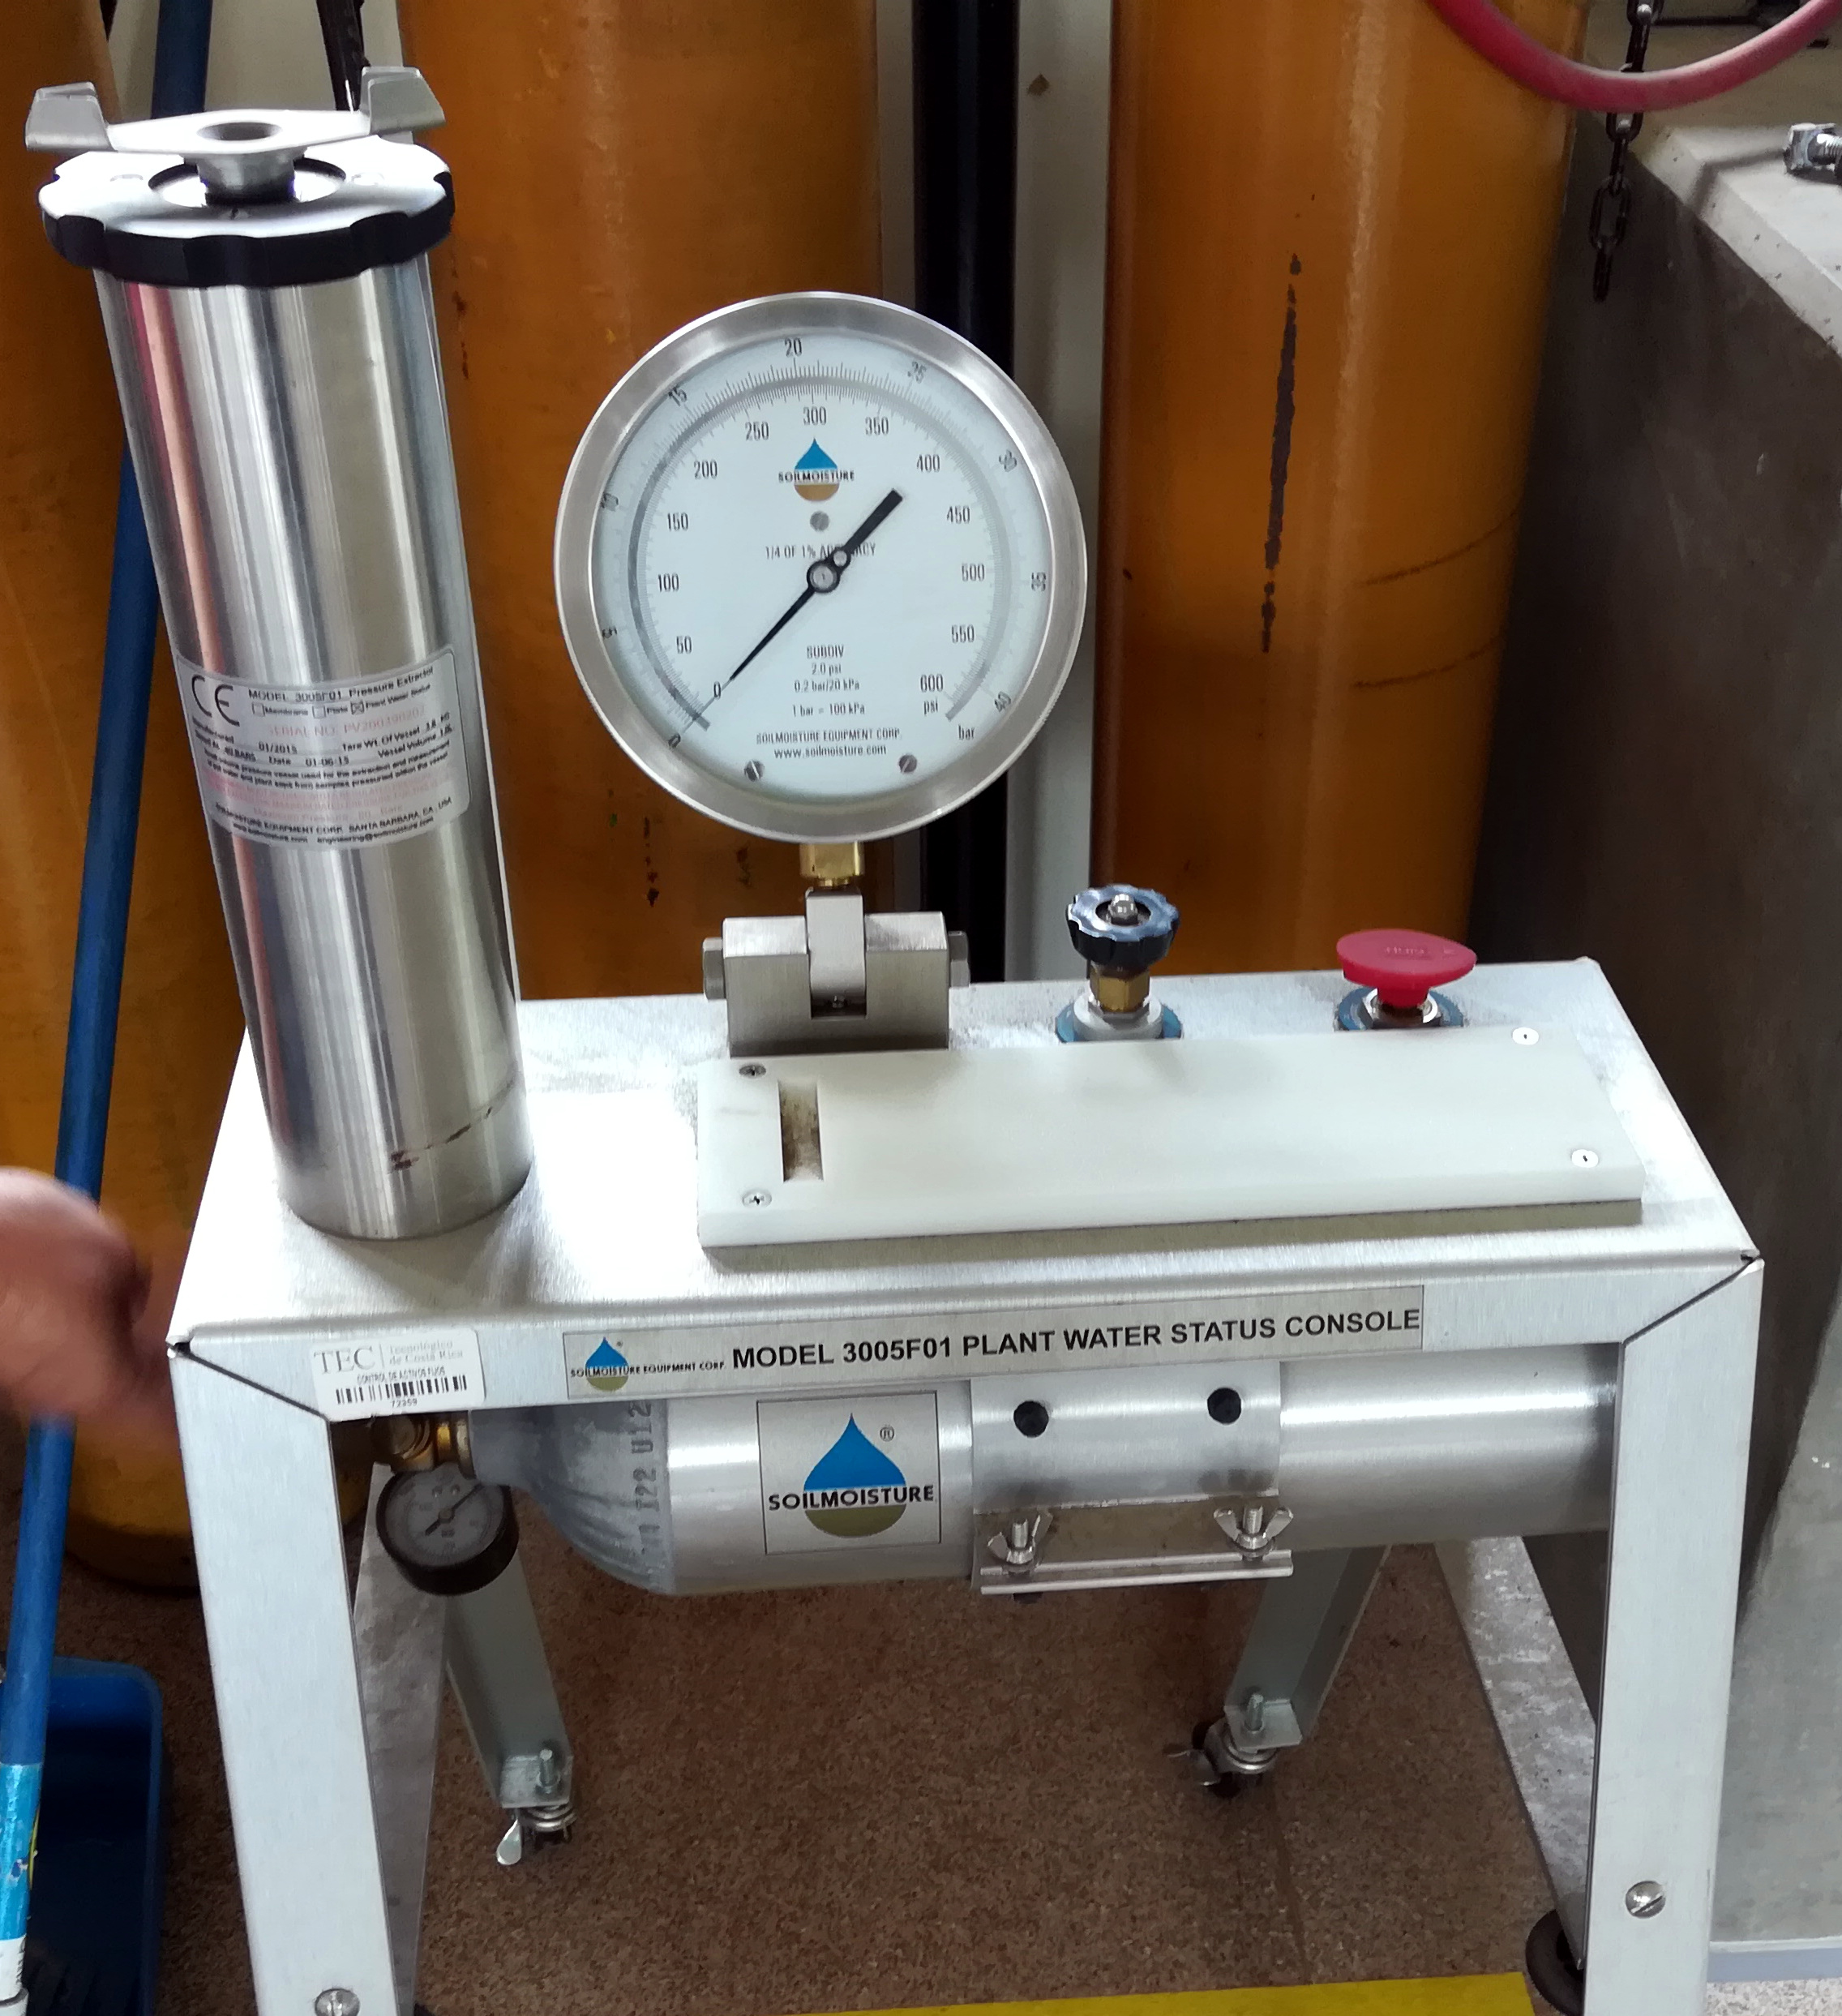
\includegraphics[width =\tw]{pictures/bomba1.jpg}\\
          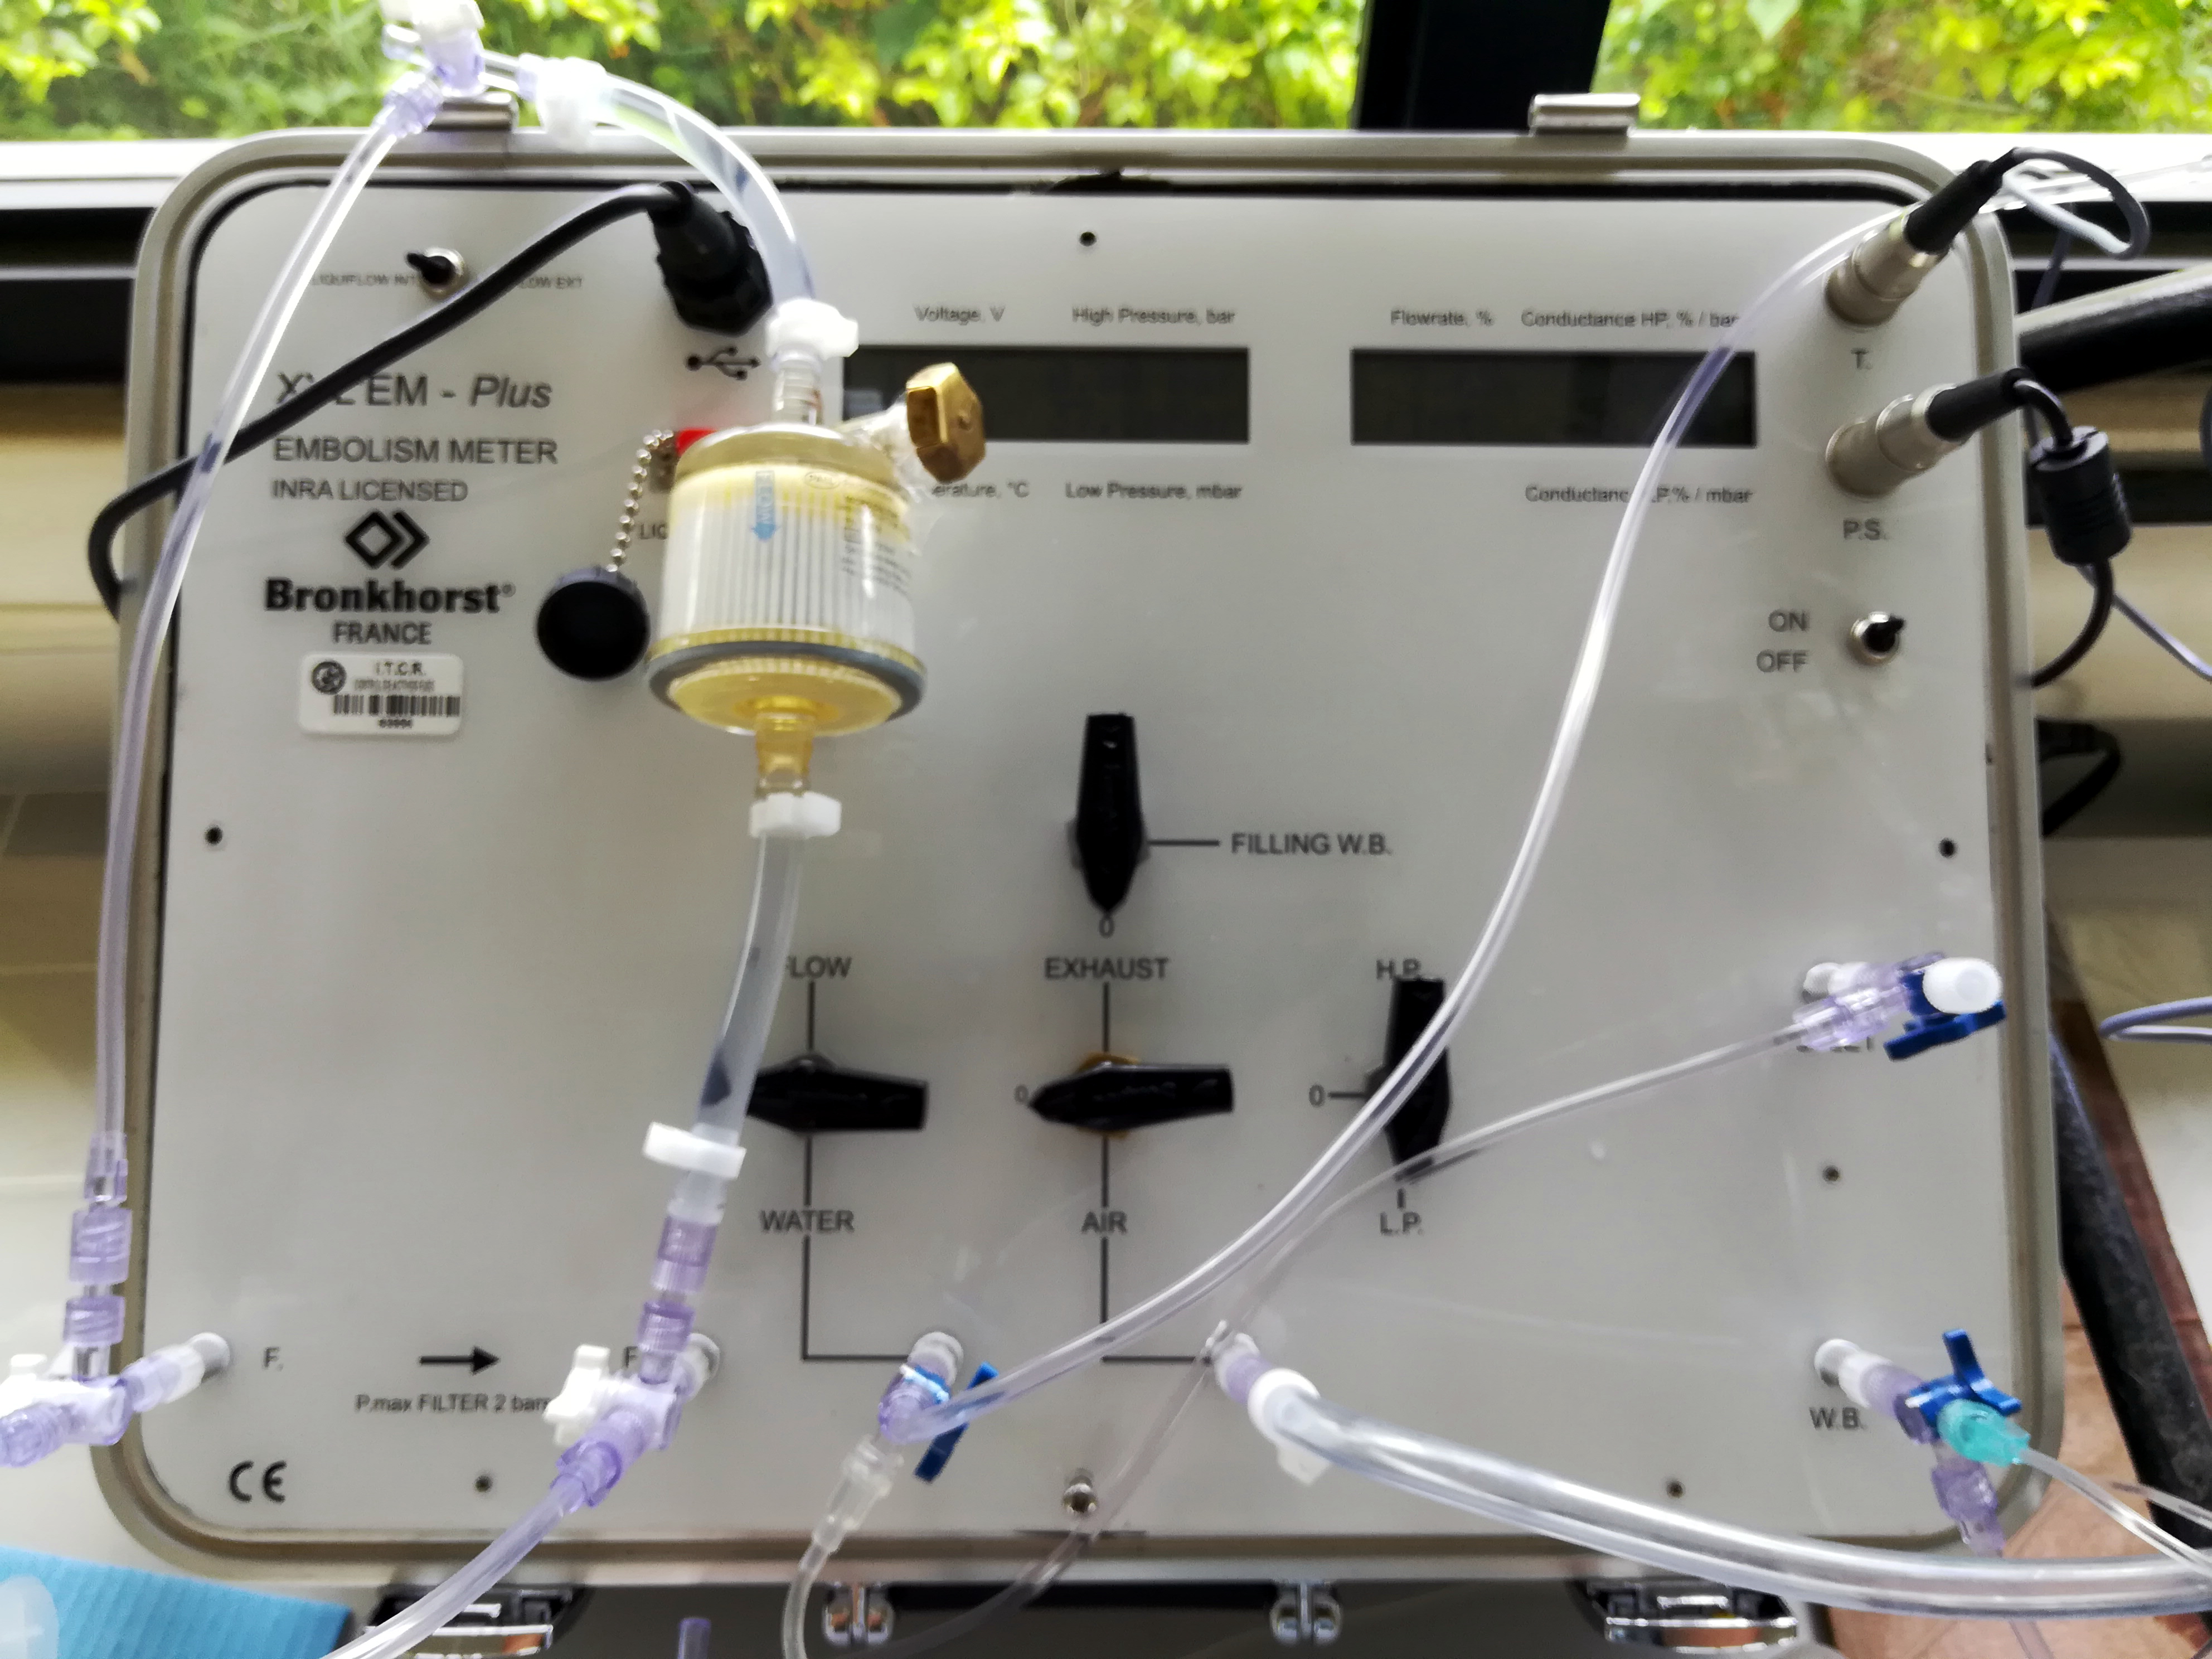
\includegraphics[width =\tw]{pictures/xylem.jpg}
		\end{minipage}	
\end{frame}

\begin{frame}
	\centering{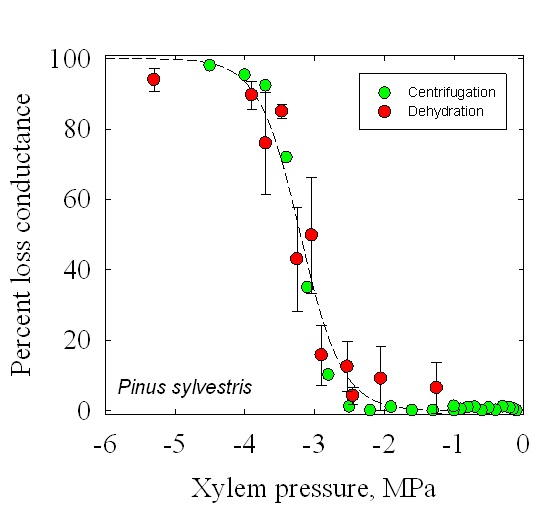
\includegraphics[width =0.6 \tw]{pictures/VC.png}}\\
    \only<1>{
	\textbf{Ejes del diagrama:}
		\begin{description}
			\item[x] Potencial hídrico del xilema []MPa]
			\item[y] Porcentaje de perdida de conductancia\\ (PLC por sus siglas en ingles) [\%]
		\end{description}}
    \only<2>{
	\textbf{Parámetros de la curva:}
		\begin{description}
			\item[P50] Potencial hídrico relacionado a una perdida 50\%\\ de la capacidad conductiva
			\item[pendiente] ¿Qué rápido ocurre la pérdida de conductividad?
		\end{description}}
	\centering{\quelle{\textbf{Ilustración:}   http://prometheuswiki.org}}
\end{frame}


\begin{frame}
	\frametitle{Métodos de medición}
	\begin{description}[<+-| alert@+>]
		\item[\textbf{Bench Dehydration}] El "método clásico" - potenciales de agua medidos por la bomba de Scholander y conductividades medidos por un aparato de Sperry o el XylEm usando muestras que se seca en el aire
		\item[\textbf{Double ended pressure sleeve}] Inducción de embolias por presión positiva aplicada en una cámara de presión que contiene la muestra
		\item[\textbf{Cavitron}] Muestra en una centrifuga, inducción de embolias y de gradiente de presión usando la fuerza centrípeta
	\end{description}
\end{frame}


\begin{frame}
	\frametitle{El valor de curvas de vulnerabilidad}
\begin{block}{\textbf{Informaciones sobre la \alert{estrategía hidráulica} de plantas}}
		\begin{itemize}	[<+-| alert@+>]		
			\item Parámetros determinan hasta que potencial hídrico una planta está capaz de mantener el flujo de agua hacia las hojas
			\item[\Rar] Adaptabilidad de una especies/un genotipo a un clima más caliente y seco
			\item[\Rar] P50: criterio muy relevante para el mejoramiento genético de árboles forestales o frutales
		\end{itemize}
\end{block}
\end{frame}

\begin{frame}
	\frametitle{Ventajas y desventajas}
	\begin{itemize}
		\item \textbf{Ventajas de curvas de vulnerabilidad}
		\begin{itemize}			
			\item Parámetros con interpretación inmediata mecanística
			\item Fuerte predictor de respuestas de plantas a sequía 
		\end{itemize}
		\item \textbf{Desventajas de curvas de vulnerabilidad}
		\begin{itemize}
			\item Medición muy compleja, requiere mucho tiempo
			\item Requiere equipo caro
			\item Algunos métodos están susceptibles a artefactos de medición relacionados a la longitud de vasos 
			\item Baja escalabilidad  
		\end{itemize}
	\end{itemize}
\end{frame}

\begin{frame}
	\frametitle{Alternativas}
	\begin{itemize}
		\item \Blue{Curvas de presión/volumen}\\ \rar\ medición directa del punto de perdida de turgencia

		\item \Blue{Osmómetro}\\ \rar\ estimación del punto de perdida de turgencia
		\item \Blue{Contenido relativo de agua de hojas}\\ \rar\ relacionado con mortalidad por sequía
	\end{itemize}
\end{frame}

 %%%%%%%%%%%%%%%%%%%%%%%%%%%%%%%%%%%%%%%%%%%%%%%%%%%%%%%%%%%%%%%%%%%%%%%%%%%%%%%%%%%%%%
\section{Referencias}
%%%%%%%%%%%%%%%%%%%%%%%%%%%%%%%%%%%%%%%%%%%%%%%%%%%%%%%%%%%%%%%%%%%%%%%%%%%%%%%%%%%%%%
\begin{frame}%[allowframebreaks]
\frametitle{Referencias}\label{bib}
\color{black}
\begin{changemargin}{-1.5em}{-1.5em}
 { \footnotesize \justifying
\begin{itemize}
\item \textbf{Campbell et al. (2006)}. \textit{Biology: Australian Version}. New South Wales, Australia: Prentice Education Australia.
 \item \textbf{Hacke U. G., Sperry J. S., 2001:} \textit{Functional and ecological xylem anatomy}. Perspectives in plant ecology, evolution and systematics 4.2: 97--115.
\item \textbf{Sperry J. S., et al., 2006:} \textit{Size and function in conifer tracheids and angiosperm vessels}. American Journal of Botany 93.10: 1490--1500.
 \item \textbf{Stroock A. D. et al., 2014:} \textit{The physicochemical hydrodynamics of vascular plants}. Annual Review of Fluid Mechanics 46: 615--642.
 \item \textbf{Taiz, L., \& Zeiger, E. (2002).} \textit{Plant Physiology,} Sinauer Associates.
 \item   \textbf{Tyree, M. T. \& Zimmermann, M. H. (2002).}\textit{ Xylem structure and the ascent of sap.} Springer, Berlin, Heidelberg.
 \item \textbf{Zimmermann M. H., McDonough J. 1978:} \textit{Dysfunction in the flow of food.} Plant disease, an advanced treatise 3: 117--140.
 \end{itemize}
} 

\end{changemargin}
\end{frame}
\end{document}
